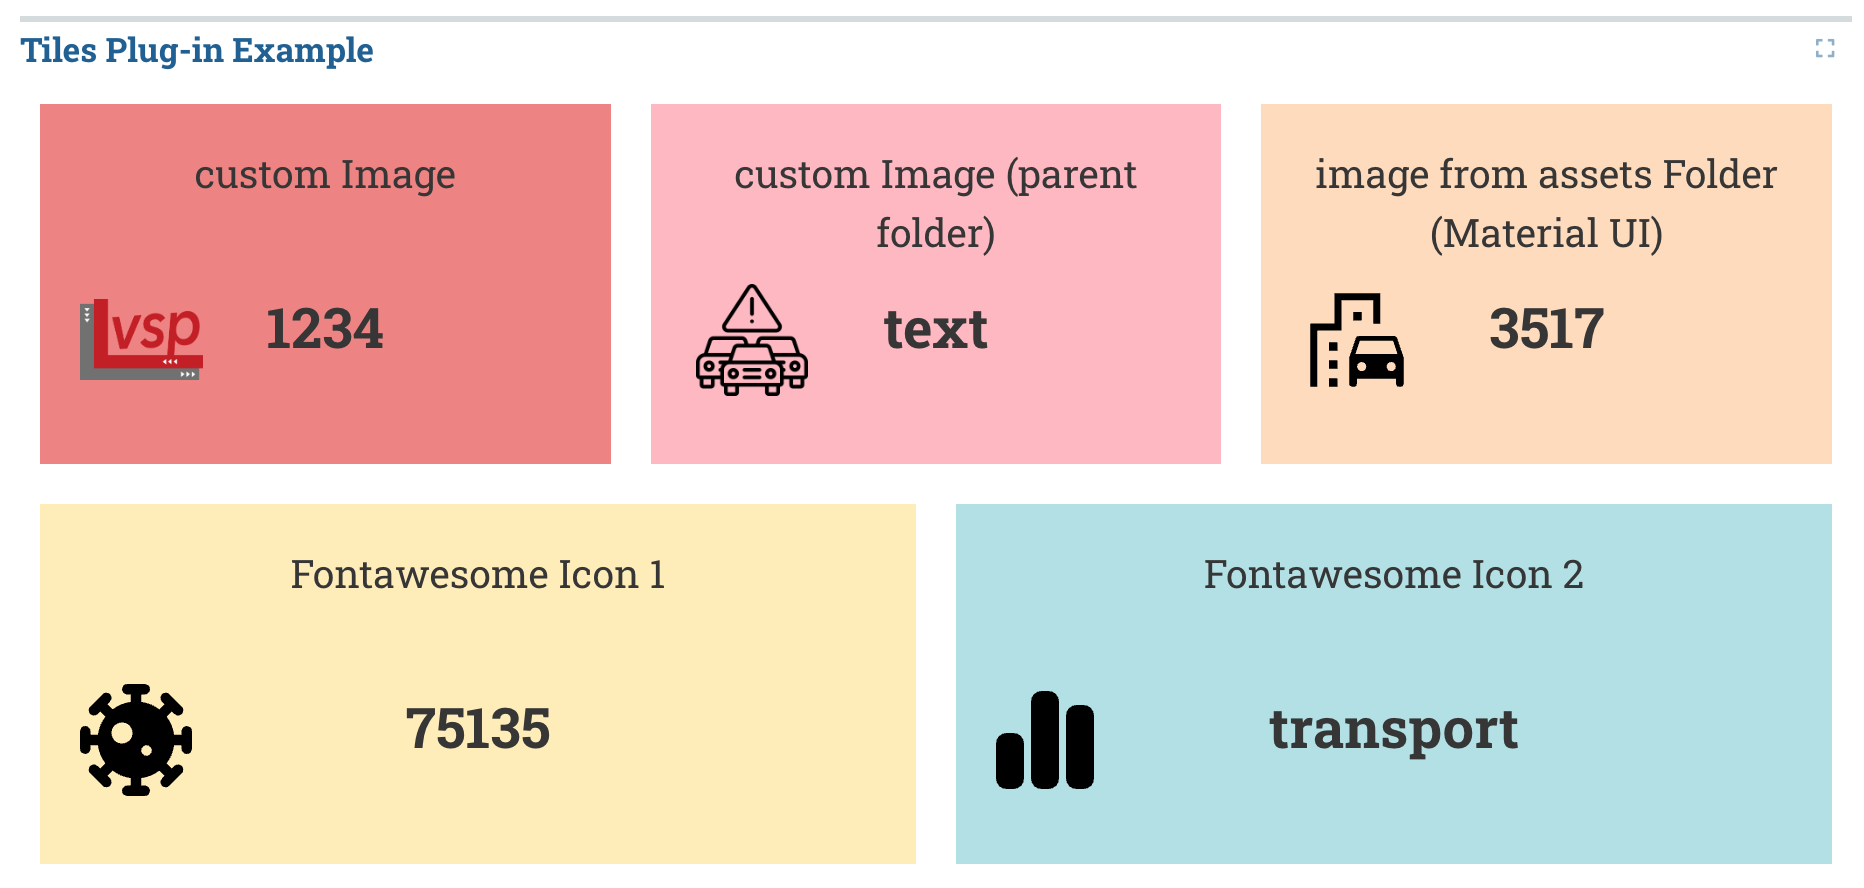
\includegraphics{assets/tiles_light_mode.png} \emph{Tiles}

The Tiles plug in displays key data for a good overview.

\hypertarget{usage}{%
\subsection{Usage}\label{usage}}

The tiles plug-in can only be included as panels in \textbf{Dashboards}.
See Dashboard documentation for general tips on creating dashboard
configurations.

\begin{itemize}
\tightlist
\item
  Each table viewer panel is defined inside a \textbf{row} in a
  \texttt{dashboard-*.yaml} file.
\item
  Use panel \texttt{type:\ csv} in the dashboard configuration.
\item
  Standard title, description, and width fields define the frame.
\end{itemize}

\begin{center}\rule{0.5\linewidth}{0.5pt}\end{center}

\hypertarget{sample-dashboard.yaml-config-snippet}{%
\subsubsection{Sample dashboard.yaml config
snippet}\label{sample-dashboard.yaml-config-snippet}}

\begin{Shaded}
\begin{Highlighting}[]
\FunctionTok{layout}\KeywordTok{:}
\AttributeTok{  }\FunctionTok{row1}\KeywordTok{:}
\AttributeTok{    }\KeywordTok{{-}}\AttributeTok{ }\FunctionTok{type}\KeywordTok{:}\AttributeTok{ }\StringTok{\textquotesingle{}tiles\textquotesingle{}}
\AttributeTok{      }\FunctionTok{title}\KeywordTok{:}\AttributeTok{ Tiles Plug{-}in Example}
\AttributeTok{      }\FunctionTok{dataset}\KeywordTok{:}\AttributeTok{ }\StringTok{\textquotesingle{}data.csv\textquotesingle{}}
\end{Highlighting}
\end{Shaded}

\begin{center}\rule{0.5\linewidth}{0.5pt}\end{center}

\hypertarget{csv-structure}{%
\subsubsection{CSV Structure}\label{csv-structure}}

The following .csv structure belongs to the sample image above. The
first line contains the titles, the second line the values and the third
line the names or paths of the icons. The values and the icons are not
required.

custom Image

custom Image (parent folder)

image from assets Folder (Material UI)

Fontawesome Icon 1

Fontawesome Icon 2

1234

text

3517

75135

transport

vsp\_logo.png

../warning.png

emoji\_transportation

virus-covid

chart-simple

\begin{center}\rule{0.5\linewidth}{0.5pt}\end{center}

\hypertarget{add-icons-to-the-tile}{%
\subsubsection{Add icons to the tile}\label{add-icons-to-the-tile}}

There are three ways to add icons. When adding icons, these three
options are also checked in this order:

\begin{enumerate}
\def\labelenumi{\arabic{enumi}.}
\item
  \textbf{Custom Icons:} To add your own icons, the file must be in the
  same directory and the relative path (including extension) must be
  specified in the .csv file.
\item
  \textbf{Predefined Icons:} See
  \protect\hyperlink{ux5cux23ux5cux23predefined-icons}{Predefined
  Icons}. For adding only the name (without extension) must be
  specified.
\item
  \textbf{Font Awesome Free Icons:} For adding these icons only the name
  must be specified. An overview of the available icons can be found
  \href{https://fontawesome.com/search?o=r\&m=free\&s=solid}{here}. Only
  the icons from the Solid series will work.
\end{enumerate}

\begin{center}\rule{0.5\linewidth}{0.5pt}\end{center}

\hypertarget{predefined-icons}{%
\subsubsection{Predefined Icons}\label{predefined-icons}}

\begin{longtable}[]{@{}cl@{}}
\toprule()
Name & Icon \\
\midrule()
\endhead

\includegraphics{assets/departure_board.svg} & departure\_board \\

\includegraphics{assets/electric_car.svg} & electric\_car \\

\includegraphics{assets/route.svg} & route \\

\includegraphics{assets/local_gas_station.svg} & local\_gas\_station \\
And many more\ldots{} & And many more\ldots{} \\
\bottomrule()
\end{longtable}

For a complete overview, you can check
\href{https://github.com/simwrapper/simwrapper/tree/overview-panel/src/assets/tile-icons}{here}.
You can also add more icons and save them in this folder. Please use
this \href{https://fonts.google.com/icons}{link} and select these
options for a consistent design: Grade: 0; Fill: true; Weight: 400;
Optical Size: 48px.

\begin{center}\rule{0.5\linewidth}{0.5pt}\end{center}

\hypertarget{table-viewer-properties}{%
\subsubsection{Table viewer properties}\label{table-viewer-properties}}

Tiles plug-in properties:

\textbf{dataset:} String. The filepath containing the csv-file. The
first row describes the header text and the second row describes the
values
